% ltex: language=it
\chapter{Intro}\label{chap:intro} % (fold)
\section{Introduzione}\label{sec:introduzione} % (fold)
Ogni imprese o istituzione, sia pubblica che privata, si struttura e si organizza secondo la propria missione per conseguire gli \textbf{obiettivi} identificati:
\begin{itemize}
    \item \textbf{Azienda industriale privata}: ottenere utili tramite la produzione e vendita di una ben definita classe di prodotti a una classe di clienti;
    \item \textbf{Azienda pubblica di servizi}: erogare un insieme di servizi a una classe di utenti massimizzando la qualità del servizio e minimizzandone allo stesso tempo il costo;
\end{itemize}
Per far ciò l'impresa si struttura definendo una propria \textbf{struttura organizzativa} e un insieme di \textbf{processi funzionali} che ne definiscono il comportamento.
\begin{note}
    Per capire un'azienda è fondamentale conoscerne, obiettivi, struttura organizzativa e processi funzionali
\end{note}
%
\subsection{Struttura e Processo}\label{sub:struttura_e_processo} % (fold)
Struttura e Processo\begin{definition}{Struttura Organizzativa}{}
    Suddivisione dell'impresa in differenti unità organizzative alle quali sono attribuiti compiti e obiettivi specifici che cooperano attraverso legami di tipo gerarchico e funzionale.
    \\
    I legami gerarchici nelle strutture organizzative vengono descritti tramite reticoli che delineano responsabilità e funzioni.
\end{definition}
\begin{cimage}
    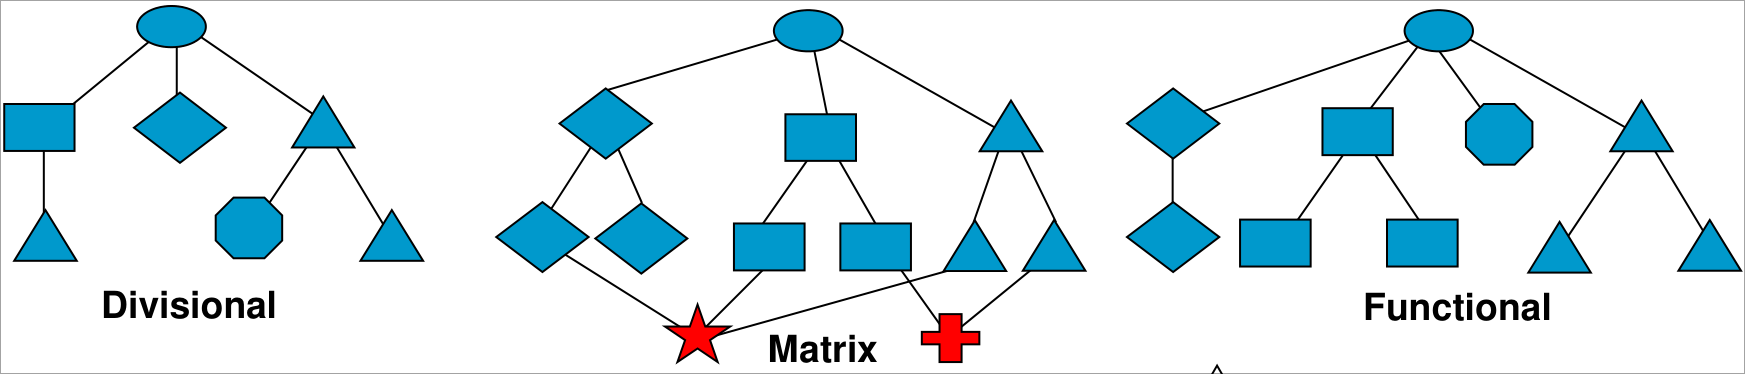
\includegraphics[width=.8\textwidth]{assets/strut-org-type.png}
\end{cimage}
\begin{description}
    \item[Divisional] Le persone vengono raggruppate in base al prodotto o servizio che forniscono, non al lavoro che svolgono.
    \item[Functional] Raggruppa le persone che svolgono compiti simili in base alla loro area di specializzazione.
        In altre parole, tutti i contabili in finanza e tutti i marketer nel marketing.
        I manager guidano ogni area e riferiscono a un direttore o dirigente che potrebbe supervisionare più dipartimenti.
    \item[Matrix] È un ibrido delle strutture funzionali e divisionali.
        Può coinvolgere dipendenti che riferiscono a capi diversi a seconda del loro attuale incarico.
\end{description}
\begin{note}
    \begin{cimage}
        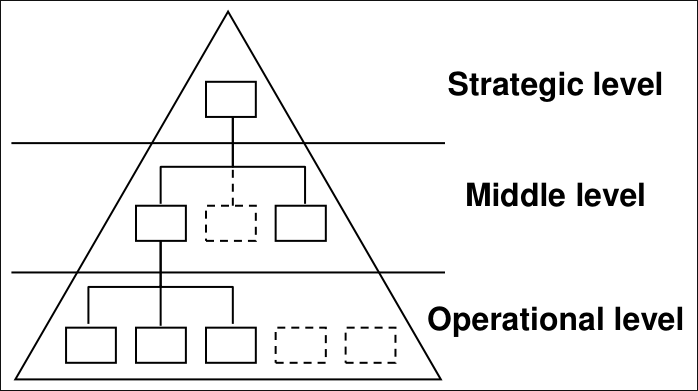
\includegraphics[width=.4\textwidth]{assets/strut-org-lvl-visual.png}
    \end{cimage}
    È consolidata la suddivisione su tre livelli delle mansioni aziendali:
    \begin{itemize}
        \item \textbf{strategic}: si concentra sulle attività necessarie per garantire un posizionamento competitivo e una strategia a lungo termine;
        \item \textbf{middle}: implementa i piani strategici e garantisce che le attività quotidiane siano conformi alla strategia aziendale;
        \item \textbf{operational}: è legato alle operazioni di breve termine di un'azienda, riguarda l'implementazione di beni e servizi;
    \end{itemize}
\end{note}
\begin{definition}{Processo}{}
    Insieme delle attività tra loro interrelate, finalizzate alla realizzazione di un risultato definito e misurabile che contribuisce al raggiungimento della missione dell'azienda.
    \\
    L'analisi dell'azienda come insiemi di processi determina una vista ortogonale rispetto a quella basata sulla sua organizzazione e sulle funzioni svolte dalle diverse divisioni.
\end{definition}
\begin{note}
    La produzione di prodotti/servizi in genere richiede il coinvolgimento di più unità organizzative, attraverso una distribuzione di compiti e responsabilità, spesso codificata in norme che regolano il processo.
    \\
    Il processo in questa accezione è quindi l'elemento di omogeneizzazione dell'organizzazione.
\end{note}
% subsection Struttura e Processo (end)
% section Introduzione (end)
% chapter Intro (end)
